\section{Fast R-CNN architecture and training}

\figref{arch} illustrates the Fast R-CNN architecture.
A Fast R-CNN network takes as input an entire image and a set of object proposals.
The network first processes the whole image with several convolutional (\emph{conv}) and max pooling layers to produce a conv feature map.
Then, for each object proposal a region of interest (\emph{\roi}) pooling layer extracts a fixed-length feature vector from the feature map.
Each feature vector is fed into a sequence of fully connected (\emph{fc}) layers that finally branch into two sibling output layers: one that produces softmax probability estimates over $K$ object classes plus a catch-all ``background'' class and another layer that outputs four real-valued numbers for each of the $K$ object classes.
Each set of $4$ values encodes refined bounding-box positions for one of the $K$ classes.

\begin{figure}[t!]
\centering
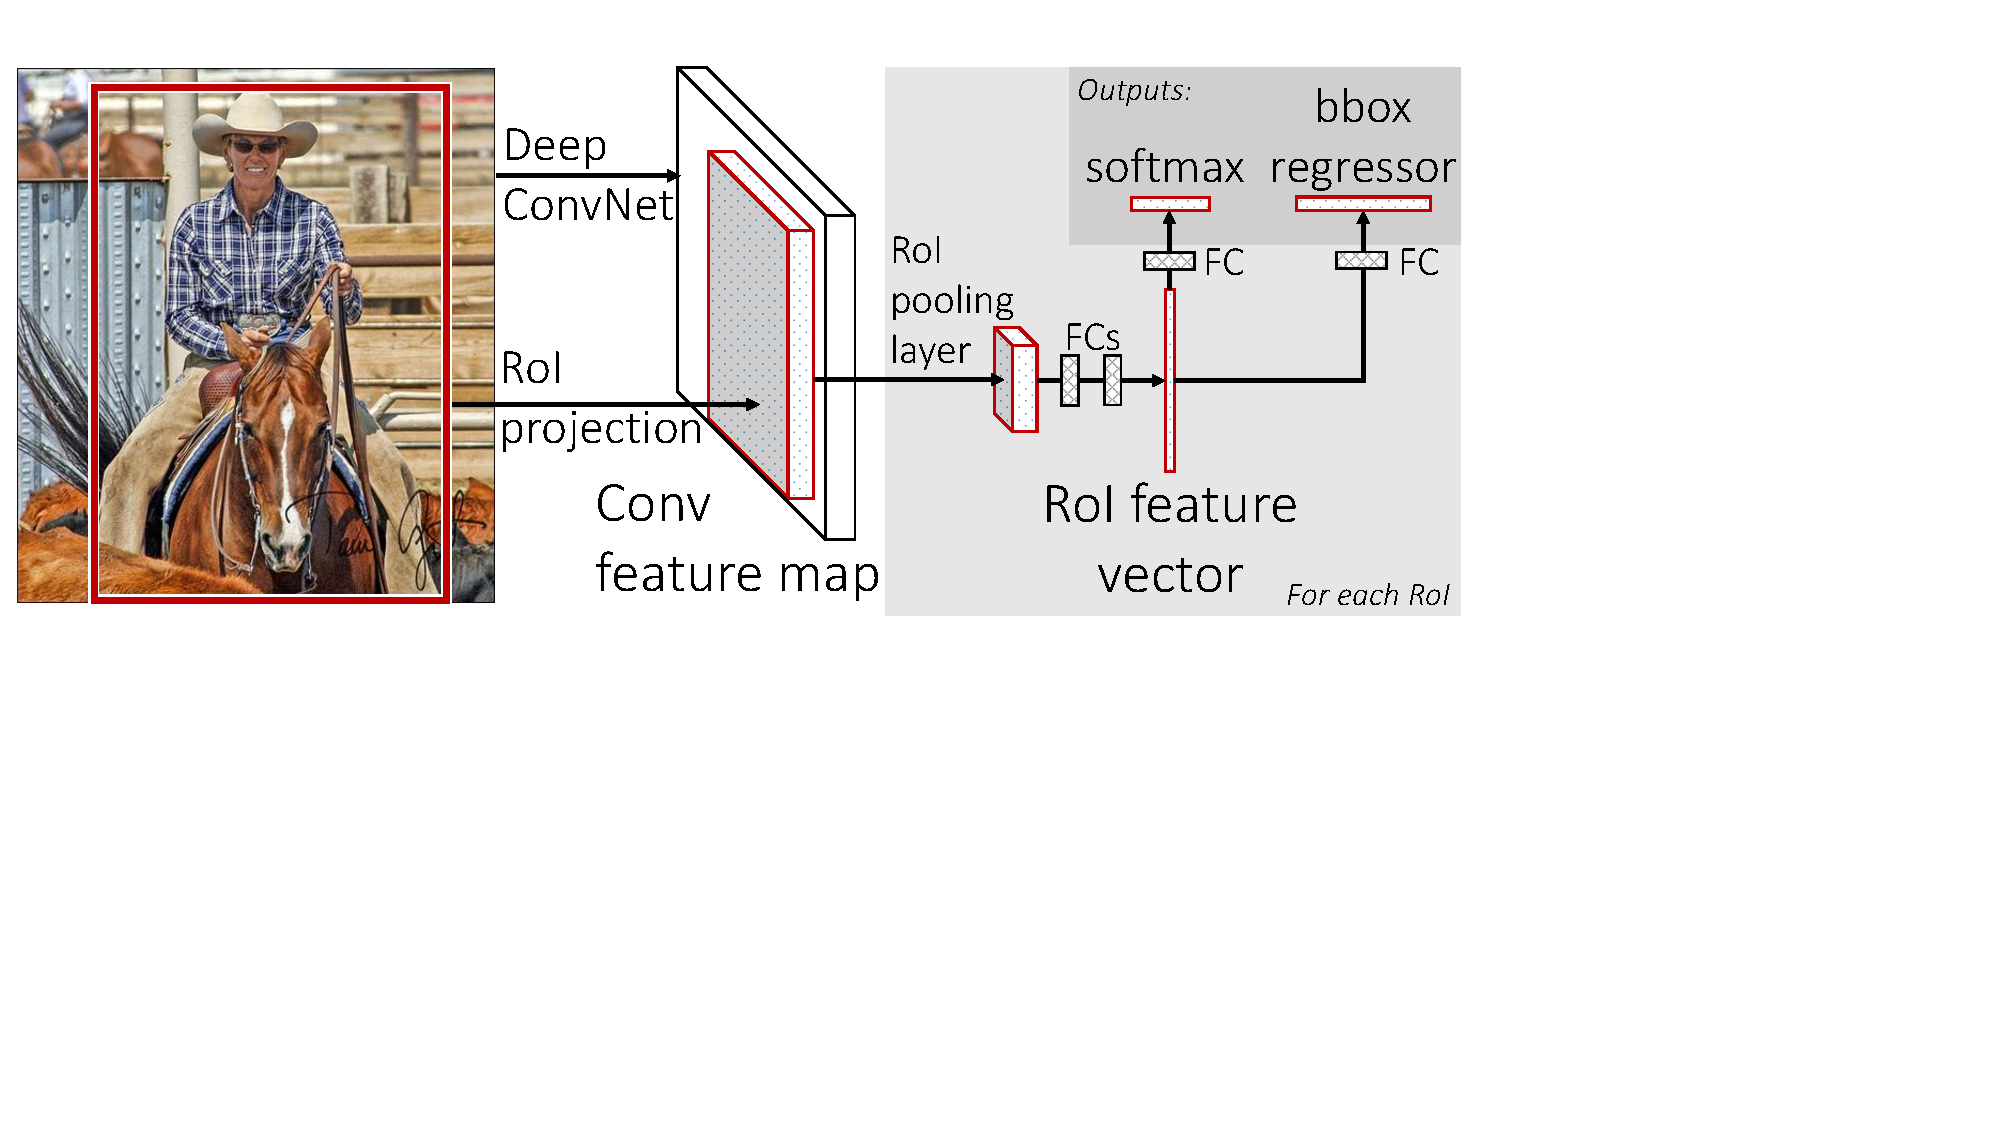
\includegraphics[width=1\linewidth,trim=0 24em 25em 0, clip]{figs/arch.pdf}
%\vspace{-1em}
\caption{Fast R-CNN architecture. An input image and multiple regions of interest ({\roi}s) are input into a fully convolutional network. Each \roi is pooled into a fixed-size feature map and then mapped to a feature vector by fully connected layers (FCs). The network has two output vectors per \roi: softmax probabilities and per-class bounding-box regression offsets. The architecture is trained end-to-end with a multi-task loss.}
\figlabel{arch}
\end{figure}


\subsection{The \roi pooling layer}
The \roi pooling layer uses max pooling to convert the features inside any valid region of interest into a small feature map with a fixed spatial extent of $H \times W$ (\eg, $7 \times 7$), where $H$ and $W$ are layer hyper-parameters that are independent of any particular \roi.
In this paper, an \roi is a rectangular window into a conv feature map.
Each \roi is defined by a four-tuple $(r, c, h, w)$ that specifies its top-left corner $(r, c)$ and its height and width $(h, w)$.

\roi max pooling works by dividing the $h \times w$ RoI window into an $H \times W$ grid of sub-windows of approximate size $h / H \times w / W$ and then max-pooling the values in each sub-window into the corresponding output grid cell.
Pooling is applied independently to each feature map channel, as in standard max pooling.
The \roi layer is simply the special-case of the spatial pyramid pooling layer used in SPPnets \cite{he2014spp} in which there is only one pyramid level.
We use the pooling sub-window calculation given in \cite{he2014spp}.


%The region of interest (\roi) pooling layer is a simplified version of the spatial pyramid pooling used in SPPnet \cite{he2014spp}, in which our ``pyramid'' has only a single level.
%A \roi pooling layer takes as input $N$ feature maps and a list of $R$ regions of interest; typically $R \gg N$.
%The $N$ feature maps are supplied by the last conv layer of the network and each is a multi-dimensional array of size $H \times W \times C$, with $H$ rows, $W$ columns, and $C$ channels.
%Each \roi is a tuple $(n, r, c, h, w)$ that specifies a feature map index $n \in \{0, \ldots, N-1\}$, the \roi's top-left location $(r, c)$, and its height and width $(h, w)$.
%\roi pooling layers output max-pooled feature maps with spatial extent $H' \times W'$ and the original $C$ channels ($H' \le H$ and $W' \le W$).
%
%For each of the $R$ {\roi}s, the \roi pooling layer performs max pooling over $H'W'$ output bins.
%The bin sizes ($\approx h/H' \times w/W'$) are adaptively set such that they tile the $h \times w$ rectangle in the indexed feature map.
%We use the adaptive bin-size calculation given in \cite{he2014spp}.

\subsection{Initializing from pre-trained networks}
We experiment with three pre-trained ImageNet \cite{imagenet_cvpr09} networks, each with five max pooling layers and between five and thirteen conv layers (see \secref{setup} for network details).
When a pre-trained network initializes a Fast R-CNN network, it undergoes three transformations.

First, the last max pooling layer is replaced by a \roi pooling layer that is configured by setting $H$ and $W$ to be compatible with the net's first fully connected layer (\eg, $H = W = 7$ for \vggsixteen).

Second, the network's last fully connected layer and softmax (which were trained for 1000-way ImageNet classification) are replaced with the two sibling layers described earlier (a fully connected layer and softmax over $K + 1$ categories and category-specific bounding-box regressors).

Third, the network is modified to take two data inputs: a list of images and a list of {\roi}s in those images.
%Each \roi four-tuple is augmented with the index $n \in \{0,\ldots,N-1\}$ of its image in the input batch.
%Typical values used during training are $N = 2$ and $R = 128$.
%The number of {\roi}s can change dynamically from batch to batch, as can the resolution of the input images: all conv layers reshape on-the-fly in proportion to the input resolution \cite{lecun94}.
%and the \roi pooling layer produces fixed-size outputs.
%During training $N$ will be small (\eg, 2) and each batch comprises independently sampled images to be used in one SGD update.
%The $R$ regions of interest will be 128 {\roi}s sampled from the $N$ input images.
%During testing $N$ will either be 1, in the case of processing an image at a single scale, or a small number (\eg, 5) in the case that the test image is processed at multiple scales.

\subsection{Fine-tuning for detection}
Training all network weights with back-propagation is an important capability of Fast R-CNN.
First, let's elucidate why SPPnet is unable to update weights below the spatial pyramid pooling layer.

The root cause is that back-propagation through the SPP layer is highly inefficient when each training sample (\ie \roi) comes from a different image, which is exactly how R-CNN and SPPnet networks are trained.
The inefficiency stems from the fact that each \roi may have a very large receptive field, often spanning the entire input image.
Since the forward pass must process the entire receptive field, the training inputs are large (often the entire image).

We propose a more efficient training method that takes advantage of feature sharing during training.
In Fast R-CNN training, stochastic gradient descent (SGD) mini-batches are sampled hierarchically, first by sampling $N$ images and then by sampling $R/N$ {\roi}s from each image.
Critically, {\roi}s from the same image share computation and memory in the forward and backward passes.
Making $N$ small decreases mini-batch computation.
For example, when using $N = 2$ and $R = 128$, the proposed training scheme is roughly 64\X faster than sampling one {\roi} from $128$ different images (\ie, the R-CNN and SPPnet strategy).

One concern over this strategy is it may cause slow training convergence because {\roi}s from the same image are correlated.
This concern does not appear to be a practical issue and we achieve good results with $N = 2$ and $R = 128$ using fewer SGD iterations than R-CNN.

In addition to hierarchical sampling, Fast R-CNN uses a streamlined training process with one fine-tuning stage that jointly optimizes a softmax classifier and bounding-box regressors, rather than training a softmax classifier, SVMs, and regressors in three separate stages \cite{girshick2014rcnn,he2014spp}.
The components of this procedure (the loss, mini-batch sampling strategy, back-propagation through \roi pooling layers, and SGD hyper-parameters) are described below.

\paragraph{Multi-task loss.}
A Fast R-CNN network has two sibling output layers.
The first outputs a discrete probability distribution (per \roi), $p = (p_0,\ldots,p_K)$, over $K + 1$ categories.
As usual, $p$ is computed by a softmax over the $K + 1$ outputs of a fully connected layer.
The second sibling layer outputs bounding-box regression offsets, $t^{k} = \left(t^{k}_\textrm{x}, t^{k}_\textrm{y}, t^{k}_\textrm{w}, t^{k}_\textrm{h}\right)$, for each of the $K$ object classes, indexed by $k$.
We use the parameterization for $t^{k}$ given in \cite{girshick2014rcnn}, in which $t^k$ specifies a scale-invariant translation and log-space height/width shift relative to an object proposal.

Each training \roi is labeled with a ground-truth class $u$ and a ground-truth bounding-box regression target $v$.
We use a multi-task loss $L$ on each labeled {\roi} to jointly train for classification and bounding-box regression:
\begin{equation}
\eqlabel{loss}
L(p, u, t^u, v) = L_\textrm{cls}(p, u) + \lambda [u \ge 1] L_\textrm{loc}(t^u, v),
\end{equation}
in which $L_\textrm{cls}(p, u) = -\log p_u$ is log loss for true class $u$.

The second task loss, $L_{\textrm{loc}}$, is defined over a tuple of true bounding-box regression targets for class $u$, $v = (v_\textrm{x}, v_\textrm{y}, v_\textrm{w}, v_\textrm{h})$, and a predicted tuple $t^u = (t^u_\textrm{x}, t^u_\textrm{y}, t^u_\textrm{w}, t^u_\textrm{h})$, again for class $u$.
The Iverson bracket indicator function $[u \ge 1]$ evaluates to 1 when $u \ge 1$ and 0 otherwise.
By convention the catch-all background class is labeled $u = 0$.
For background {\roi}s there is no notion of a ground-truth bounding box and hence $L_\textrm{loc}$ is ignored.
For bounding-box regression, we use the loss
\begin{equation}
L_\textrm{loc}(t^u, v) = \sum_{i \in \{\textrm{x},\textrm{y},\textrm{w},\textrm{h}\}} \textrm{smooth}_{L_1}(t^u_i - v_i),
\end{equation}
in which
\begin{equation}
\eqlabel{smoothL1}
  \textrm{smooth}_{L_1}(x) =
  \begin{cases}
    0.5x^2& \text{if } |x| < 1\\
    |x| - 0.5& \text{otherwise},
  \end{cases}
\end{equation}
is a robust $L_1$ loss that is less sensitive to outliers than the $L_2$ loss used in R-CNN and SPPnet.
When the regression targets are unbounded, training with $L_2$ loss can require careful tuning of learning rates in order to prevent exploding gradients.
\eqref{smoothL1} eliminates this sensitivity.

The hyper-parameter $\lambda$ in \eqref{loss} controls the balance between the two task losses.
We normalize the ground-truth regression targets $v_i$ to have zero mean and unit variance.
All experiments use $\lambda = 1$.

We note that \cite{erhan2014scalable} uses a related loss to train a class-agnostic object proposal network.
Different from our approach, \cite{erhan2014scalable} advocates for a two-network system that separates localization and classification.
OverFeat \cite{overfeat}, R-CNN \cite{girshick2014rcnn}, and SPPnet \cite{he2014spp} also train classifiers and bounding-box localizers, however these methods use stage-wise training, which we show is suboptimal for Fast R-CNN (\secref{multitask}).

\paragraph{Mini-batch sampling.}
During fine-tuning, each SGD mini-batch is constructed from $N = 2$ images, chosen uniformly at random (as is common practice, we actually iterate over permutations of the dataset).
We use mini-batches of size $R = 128$, sampling $64$ {\roi}s from each image.
As in \cite{girshick2014rcnn}, we take 25\% of the {\roi}s from object proposals that have intersection over union (IoU) overlap with a ground-truth bounding box of at least $0.5$.
These {\roi}s comprise the examples labeled with a foreground object class, \ie $u \ge 1$.
%In cases of multiple overlap, the label comes from the ground-truth bounding box with which the sampled \roi has maximum IoU overlap.
The remaining {\roi}s are sampled from object proposals that have a maximum IoU with ground truth in the interval $[0.1, 0.5)$, following \cite{he2014spp}.
These are the background examples and are labeled with $u = 0$.
The lower threshold of $0.1$ appears to act as a heuristic for hard example mining \cite{lsvm-pami}.
During training, images are horizontally flipped with probability $0.5$.
No other data augmentation is used.%, though it would likely help.

\paragraph{Back-propagation through \roi pooling layers.}
%Fast R-CNN mini-batches start from whole images and hence contain all information needed to back-propagate derivatives from the loss function to the image.
%Back-propagation routes derivatives through the \roi pooling layer, as described below.
%Unlike SPPnet, we are able to fine-tuning all layers of the network because mini-batches start from whole images and hence posses the information needed to backpropagate derivatives from the loss to the image.
%Unlike SPPnet, we are able to fine-tune all layers of the network because mini-batches are constructed by first sampling images and then sampling {\roi}s within those images, rather than training from a set of pre-computed feature vectors.

%During the forward pass, an image list of $N = 2$ images is expanded by the \roi pooling layer into a mini-batch of size $R = 128$.
%The multi-task loss $L$ is averaged over the $R$ outputs.
%During back-propagation, derivatives flow through the \roi pooling layer.

Back-propagation routes derivatives through the \roi pooling layer.
For clarity, we assume only one image per mini-batch ($N=1$), though the extension to $N > 1$ is straightforward because the forward pass treats all images independently.

Let $x_i \in \mathbb{R}$ be the $i$-th activation input into the \roi pooling layer and let $y_{rj}$ be the layer's $j$-th output from the $r$-th \roi.
The \roi pooling layer computes $y_{rj} = x_{i^*(r,j)}$, in which $i^*(r,j) = \argmax_{i' \in \mathcal{R}(r,j)} x_{i'}$.
$\mathcal{R}(r,j)$ is the index set of inputs in the sub-window over which the output unit $y_{rj}$ max pools.
A single $x_i$ may be assigned to several different outputs $y_{rj}$.

The \roi pooling layer's \texttt{backwards} function computes partial derivative of the loss function with respect to each input variable $x_i$ by following the argmax switches:
\begin{equation}
  \frac{\partial L}{\partial x_i} = \sum_{r} \sum_{j}
  \left[i = i^*(r,j)\right] \frac{\partial L}{\partial y_{rj}}.
\end{equation}
In words, for each mini-batch \roi $r$ and for each pooling output unit $y_{rj}$, the partial derivative $\partial L/\partial y_{rj}$ is accumulated if $i$ is the argmax selected for $y_{rj}$ by max pooling.
In back-propagation, the partial derivatives $\partial L/\partial y_{rj}$ are already computed by the \texttt{backwards} function of the layer on top of the \roi pooling layer.

\paragraph{SGD hyper-parameters.}
The fully connected layers used for softmax classification and bounding-box regression are initialized from zero-mean Gaussian distributions with standard deviations $0.01$ and $0.001$, respectively.
Biases are initialized to $0$.
All layers use a per-layer learning rate of 1 for weights and 2 for biases and a global learning rate of $0.001$.
When training on VOC07 or VOC12 trainval we run SGD for 30k mini-batch iterations, and then lower the learning rate to $0.0001$ and train for another 10k iterations.
When we train on larger datasets, we run SGD for more iterations, as described later.
A momentum of $0.9$ and parameter decay of $0.0005$ (on weights and biases) are used.

%We note that it is not clear a priori that constructing mini-batches from a small number of images ($N = 2$) should work.
%However, we find that training is well behaved with this parameter choice, likely because the SGD momentum has a strong enough averaging effect.



\subsection{Scale invariance}
We explore two ways of achieving scale invariant object detection: (1) via ``brute force'' learning and (2) by using image pyramids.
These strategies follow the two approaches in \cite{he2014spp}.
In the brute-force approach, each image is processed at a pre-defined pixel size during both training and testing.
The network must directly learn scale-invariant object detection from the training data.

The multi-scale approach, in contrast, provides approximate scale-invariance to the network through an image pyramid.
At test-time, the image pyramid is used to approximately scale-normalize each object proposal.
During multi-scale training, we randomly sample a pyramid scale each time an image is sampled, following \cite{he2014spp}, as a form of data augmentation.
We experiment with multi-scale training for smaller networks only, due to GPU memory limits.

\section{Fast R-CNN detection}
Once a Fast R-CNN network is fine-tuned, detection amounts to little more than running a forward pass (assuming object proposals are pre-computed).
The network takes as input an image (or an image pyramid, encoded as a list of images) and a list of $R$ object proposals to score.
At test-time, $R$ is typically around $2000$, although we will consider cases in which it is larger ($\approx$ $45$k).
When using an image pyramid, each \roi is assigned to the scale such that the scaled \roi is closest to $224^2$ pixels in area \cite{he2014spp}.
%For single-scale detection, all {\roi}s index the single image in the input batch.
%In the multi-scale case, the input batch is an image pyramid.
%Here, each \roi specifies a pyramid level $l$ and a rectangle within that level.

For each test \roi $r$, the forward pass outputs a class posterior probability distribution $p$ and a set of predicted bounding-box offsets relative to $r$ (each of the $K$ classes gets its own refined bounding-box prediction).
We assign a detection confidence to $r$ for each object class $k$ using the estimated probability $\textrm{Pr}(\textrm{class} = k~|~r) \stackrel{\Delta}{=} p_k$.
We then perform non-maximum suppression independently for each class using the algorithm and settings from R-CNN \cite{girshick2014rcnn}.

\subsection{Truncated SVD for faster detection}
\seclabel{svd}
For whole-image classification, the time spent computing the fully connected layers is small compared to the conv layers.
On the contrary, for detection the number of {\roi}s to process is large and nearly half of the forward pass time is spent computing the fully connected layers (see \figref{timing}).
Large fully connected layers are easily accelerated by compressing them with truncated SVD \cite{Denton2014SVD,Xue2013svd}.

In this technique, a layer parameterized by the $u \times v$ weight matrix $W$ is approximately factorized as
\begin{equation}
  W \approx U \Sigma_t V^T
\end{equation}
using SVD.
In this factorization, $U$ is a $u \times t$ matrix comprising the first $t$ left-singular vectors of $W$, $\Sigma_t$ is a $t \times t$ diagonal matrix containing the top $t$ singular values of $W$, and $V$ is $v \times t$ matrix comprising the first $t$ right-singular vectors of $W$.
Truncated SVD reduces the parameter count from $uv$ to $t(u + v)$, which can be significant if $t$ is much smaller than $\min(u, v)$.
To compress a network, the single fully connected layer corresponding to $W$ is replaced by two fully connected layers, without a non-linearity between them.
The first of these layers uses the weight matrix $\Sigma_t V^T$ (and no biases) and the second uses $U$ (with the original biases associated with $W$).
This simple compression method gives good speedups when the number of {\roi}s is large.


%\subsection{Sum pooling and integral images}
%For networks with many feature channels (\eg $C = 512$), \roi pooling over a large number of regions also takes a non-trivial amount of time.
%If the max operation in \roi pooling is switched to either a sum or average, then integral images can be used to pool {\roi}s more quickly.
%\todo{run experiments}
